
\section{Examples}
\label{sec:examp}
\subsection{$Q_{0}$ Horizontal}
\begin{itemize}
 \item $Q_{1}$ \bf{increasing} \normalfont


Given a parameter $a\in[0,\dfrac{\sqrt{2}}{2}]$, suppose that the types's $\theta$ are uniformly distributed in $[0,1]$ and their preferences  are given by

 $$v(q,\theta,a)= \theta(\dfrac{q^{2}}{2} - aq) + \theta + q$$

and the costs

 $$C(q,\theta,a)= -1 + 2\theta + q^{2}\theta + q(1 + a - \theta - 2a\theta).$$

Using the  Euler Equation  (\ref{euler}), the relaxed solution to the monopolist's problem is $Q_{1}(\theta)=\theta$ and the  curve $Q_{0}$ 
separating the regions $CS_{+}$ and $CS_{-}$ is given by a constant $Q_{0}(\theta)=a$, 

\newpage

\begin{center}
\begin{figure}[h!]
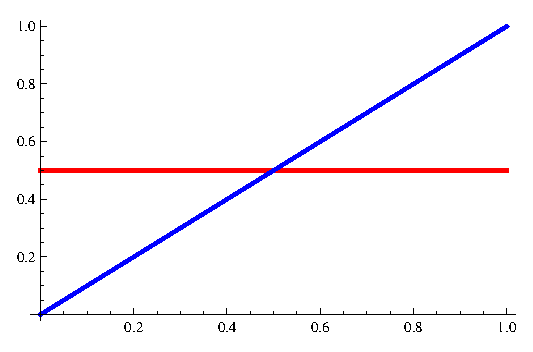
\includegraphics[scale=0.8]{hor1.eps} 
\end{figure}
Figure 1.
\end{center}

The numerical solution found by Knitro for 100 types is given by Figure 2.\\

\begin{center}
\begin{figure}[h!]
\includegraphics[scale=0.2]{knitrohor.eps} 
\end{figure}
Figure 2.
\end{center}


The numerical approach suggests that the optimal decision is a discontinuous function that consists of three parts: two flat pieces with constant decision, $q_1$ and $q_2$,
 and part of the curve relaxed $Q_{1}(\theta)$.

Thus, the optimal decision in this case, has the form $$q(\theta,a)=q_1\mathbb{I}_{[0,\theta_{d}]}(\theta,a) + q_2\mathbb{I}_{[\theta_{d}\leq \theta \leq \theta_{2}]}(\theta,a) + \theta \mathbb{I}_{[\theta_{2}\leq \theta \leq 1]}(\theta,a)$$
were $\theta_{2}=q_{2}$.\\

Monopolist's profit can be rewritten as 
\begin{equation}
 \Pi(q,\theta,a)=\int_{0}^{\theta_{d}} f(q_{1},\theta)d\theta + \int_{\theta_{d}}^{q_{2}} f(q_{2},\theta)d\theta + \int_{q_{2}}^{1} f(\theta,\theta)d\theta
\end{equation}

and the global constraint that  we consider is that the type $\theta_{2}$ does not envy $\theta_{d}$-type, which can be written, from (ISO), as
 $$\int_{\theta_{d}}^{\theta_{2}}  v_{\theta} (q_{2},s,a)  ds - \int_{\theta_{d}}^{\theta_{2}}  v_{\theta} (q(\theta_{d}),s,a) ds \geq 0$$
or, in this case
\begin{equation}
\label{iso_hor}
\int_{\theta_{d}}^{\theta_{2}}  v_{\theta} (q_{2},s,a)  ds - \int_{\theta_{d}}^{\theta_{2}}  v_{\theta} (q_{1},s,a) ds = 0
\end{equation}


\begin{center}
\begin{figure}[h!]
\includegraphics[scale=0.8]{iso_hor.eps} 
\end{figure}
Figure 3.
\end{center}



The equation (\ref{iso_hor}) implies the relationship $$q_{1}=2a-q_{2},$$

moreover, the continuity of $f(q,\theta,a)$ implies the additional condition 

$$f(q_{1},\theta_{d},a)=f(q_{2},\theta_{d},a)$$
 
which can be rewritten, using (ISO), as

\begin{equation}
\label{cont_hor}
 f(2a-q_{2},\theta_{d},a)-f(q_{2},\theta_{d},a)=0
\end{equation}

obtaining from (\ref{cont_hor}) the value for $\theta_{d}$,

$$\theta_{d}=a.$$

Finally, write the profit considering the global constraint (\ref{iso_hor}) as 
\begin{equation}
\label{lucro_hor}
\Pi(q_{2},a)=\int_{0}^{a} f(2a-q_{2},\theta,a) d\theta+ \int_{a}^{q_{2}} f(q_{2},\theta,a) d\theta+ \int_{q_{2}}^{1} f(\theta,\theta,a) d\theta
\end{equation}

In this (horizontal) case, the monopolist's problem without single-crossing was reduced to maximization problem with a single variable

\begin{equation}
\label{lucro_hor2}
 \underset{ \{q_{2}\} } { max } \, \Pi(q_{2},a)
\end{equation}
$$s.t \,\,\, a \leq q_{2}\leq 1$$

where the constraint $0 \leq \theta_{d} \leq \theta_{2} \leq 1$  was rewritten as   $a\leq q_{2}\leq 1$.\\

The expected profit $\Pi(q_{2},a)=\frac{1}{6}(1 - 6 a^3 + 6 a^2 q_{2} - q_{2}^3)$ is a strongly concave function in $q_{2}$ for all $a$, then the KKT optimality conditions are necessary and sufficient.\\

 Solving the problem  (\ref{lucro_hor2}) as a \textit{KKT system} we obtain the optimum values for $q_{1}$ and $q_{2}$ 

$$q_{1}(a)= 2a - \sqrt{2} a $$
$$q_{2}(a)= \sqrt{2} a.$$

So, the optimal decision is given by 
$$q(\theta,a)=(2a-\sqrt{2}a)\mathbb{I}_{[0\leq \theta \leq a ]} + \sqrt{2}a\mathbb{I}_{[a\leq \theta \leq \sqrt{2}a]}+\theta\mathbb{I}_{[\sqrt{2}a \leq \theta \leq 1]}$$


\begin{center}
\begin{figure}[h!]
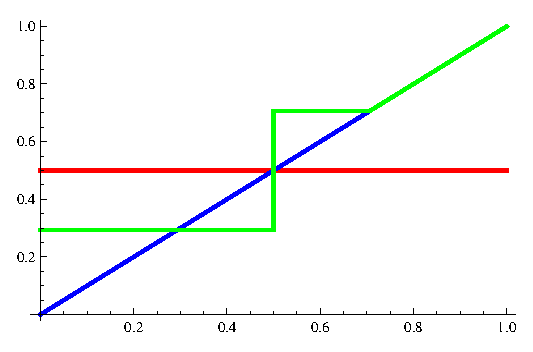
\includegraphics[scale=0.8]{completo.eps} 
\end{figure}
Figure 4.
\end{center}

\begin{center}
\begin{figure}[h!]
\includegraphics[scale=0.2]{knitroplus.eps} 
\end{figure}
Figure 5.
\end{center}




and the monopolist's expected profit from $q(\theta,a)$ is 

$$\Pi(q_{2}(a),a)=\dfrac{1}{6} (1 - 6 a^{3} + 4 \sqrt{2} a^{3})$$


%%%%%%%%% caso simetrico%%%%%%%%%%%%%%
 \vspace{1cm}

Given a parameter $a\in[\frac{3}{10},\frac{1}{2}]$, consider the types's $\theta$ uniformly distributed in $[0,1]$ with preferences given by

 $$v(q,\theta,a)= \theta(-\dfrac{q^{2}}{2} + aq) + \theta + q$$

if costs are

 $$C(q,\theta,a)= -1 - q^{2} (-1 + \theta) + 2 \theta + q (1 - \theta + a (-1 + 2 \theta)),$$


then, we get the same curves $Q_{0}$ and $Q_{1}$, but the region under the curve $Q_{0}$ is $CS_{+}$. So, we expect a decision function flat for the higher types.\\

The numerical solution found by Knitro for 100 types is given by Figure 6.\\

\begin{center}
\begin{figure}[h!]
\includegraphics[scale=0.2]{100tiposq0hor.eps} 
\end{figure}
Figure 6.
\end{center}

The numerical approach suggests that the optimal decision is a discontinuous function that consists of three parts: a first part, for the lower types, were the optimal decision is the relaxed curve $Q_{1}(\theta)$ and other two flat pieces with constant decision, $q_{1}$ and $q_{2}$, for the higher types.\\

Thus, the optimal decision in this case, has the form $$q(\theta,a)= \theta \mathbb{I}_{[0 \leq \theta \leq \theta_{1}]}(\theta,a)+ q_1\mathbb{I}_{[\theta_{1},\theta_{d}]}(\theta,a) + q_2\mathbb{I}_{[\theta_{d}\leq \theta \leq \theta_{1}]}(\theta,a) $$
were $\theta_{1}=q_{1}$.\\

Monopolist's profit can be rewritten as 
\begin{equation}
 \Pi(q,\theta,a)=\int_{0}^{q_{1}} f(\theta,\theta)d\theta + \int_{q_{1}}^{\theta_{d}} f(q_{1},\theta)d\theta + \int_{\theta_{d}}^{1} f(q_{2},\theta)d\theta
\end{equation}

From the global constraint(ISO) applied to the types $\theta_{1}$ and $\theta_{d}$ and continuity of $f$, we get the following relationships

 $$q_{1}=2a-q_{2}$$
and
$$\theta_{d}=a.$$

The monopolist's profit can be expressed as function of one  variable  


$$\Pi(q_{2},a)=\int_{0}^{2a-q_{2}} f(\theta,\theta,a) d\theta+ \int_{2a-q_{2}}^{a} f(2a-q_{2},\theta,a) d\theta+ \int_{a}^{1} f(q_2,\theta,a) d\theta$$

or

$$\Pi(q_{2},a)= \dfrac{1}{6} (2a^{3} - 6a^{2}q_{2} + 6 aq_{2}^{2} - q_{2}(-3 + 3q_{2} + q_{2}^{2})),$$

the expected profit  is a strongly concave function in $q_{2}$ for all $a\in [0, 1/2]$, then the KKT optimality conditions are necessary and sufficient.\\


Solving the problem  as a \textit{KKT system} we obtain the optimum values for $q_{1}$ and $q_{2}$ 

$$q_{1}(a)= 1 - \sqrt{2} \sqrt{(-1 + a)^2} $$
$$q_{2}(a)= -1 + \sqrt{2} \sqrt{(-1 + a)^2} + 2 a.$$

So, the optimal decision is given by 
$$q(\theta,a)=\theta \mathbb{I}_{[0\leq \theta \leq q_{1}(a) ]} + q_{1}(a)\mathbb{I}_{[q_{1}(a) \leq \theta \leq a}+ q_{2}(a) \mathbb{I}_{[a \leq \theta \leq 1]}$$


and the monopolist's expected profit from $q(\theta,a)$ is 

$$\Pi(a)=\dfrac{1}{6} (-5 + 4 \sqrt{2} \sqrt{(-1 + a)^2} + 
   2 (9 - 4 \sqrt{2} \sqrt{(-1 + a)^2}) a + 
   2 (-9 + 2 \sqrt{2} \sqrt{(-1 + a)^2}) a^2 + 6 a^3)$$

\begin{center}
\begin{figure}[h!]
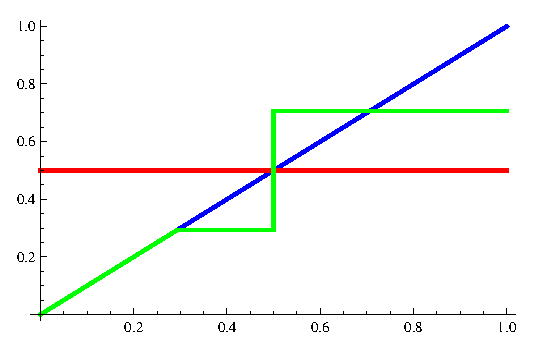
\includegraphics[scale=0.8]{hor_inv_fin.eps} 
\end{figure}
Figure 7.
\end{center}


%%%Disenhos%%%%

\item $Q_{1}$ \bf{decreasing} \\

\normalfont
With the following specifications for the distribution of types, preferences and costs  we get the same curve $Q_{0}=a$ and the relaxed solution $Q_{1}= 1 -\theta$.
 $$v(q,\theta,a)= q + \theta + (-a q + \dfrac{q^2}{2}) \theta$$


 $$C(q,\theta,a)=-1 + q^2 (-1 + \theta) + 2 \theta + q (2 + a - \theta - 2 a \theta)$$

Using the same technique as in the previous case  ((ISO) and continuity of $f$), the problem of monopoly was reduced to a one-dimensional optimization problem.\\ In the figures 8 and 9, we show the optimal decision by Knitro for the cases with $CS_{+}$ above and
 with $CS_{+}$ below, respectively. 

\begin{center}
\begin{figure}[h!]
\includegraphics[scale=0.2]{q1dec.eps} 
\end{figure}
Figure 8.
\end{center}

\newpage

\begin{center}
\begin{figure}[h!]
\includegraphics[scale=0.2]{hor_q1dec_inv.eps} 
\end{figure}
Figure 9.
\end{center}
\end{itemize}

\newpage

\subsection{$Q_{0}$ Decreasing}

Given a parameter $a\in[0,\frac{1}{3}]$, suppose that the types's $\theta$ are uniformly distributed in $[0,1]$ and their preferences  are given by

 $$v(q,\theta,a)= -(1 + a) q \theta + \frac{q^2 \theta}{2} + \frac{q \theta^{2}}{2} + q + \theta + 1,$$

and the costs

 $$C(q,\theta,a)= 2 \theta + q^2 \theta + q (1 + a - 2 \theta - 2 a \theta + \frac{3 \theta^{2}}{2}).$$

Using the  Euler Equation  (\ref{euler}), the relaxed solution and the curve $Q_{0}$ are  $Q_{1}(\theta)=1 - \theta$ 
 and $Q_{0}(\theta)=1 + a - \theta$ respectively. \\


\begin{center}
\begin{figure}[h!]
\includegraphics[scale=0.8]{q0dec.eps} 
\end{figure}
Figure 10.
\end{center}

The numerical solution found by Knitro for 100 types is given by Figure 11.\\


\begin{center}
\begin{figure}[h!]
\includegraphics[scale=0.25]{decrec.eps} 
\end{figure}
Figure 11.
\end{center}
